\documentclass[12pt]{standalone}
\usepackage[english]{babel}
\usepackage[utf8]{inputenc}

\usepackage{comment}
\usepackage{amsmath}
\usepackage{tikz}
\usepackage{circuitikz} % for circuit stuff
\usetikzlibrary{arrows.meta} % for loads
\usepackage{float}
\usetikzlibrary{positioning}
\usetikzlibrary{calc}

% Custom code for generator
\newcommand\ppbb{path picture bounding box}
\tikzset{
  do path picture/.style={%
    path picture={%
      \pgfpointdiff{\pgfpointanchor{\ppbb}{south west}}%
        {\pgfpointanchor{\ppbb}{north east}}%
      \pgfgetlastxy\x\y%
      \tikzset{x=\x/2.5,y=\y/2.5}%
      #1
    }
  },
  sin wave/.style={do path picture={    
    \draw [line cap=round] (-3/4,0)
      sin (-3/8,1/2) cos (0,0) sin (3/8,-1/2) cos (3/4,0);
  }},
	gen/.style={circle, draw=black, thick, minimum width = 2em,sin wave
	},
}

\begin{document}
	
	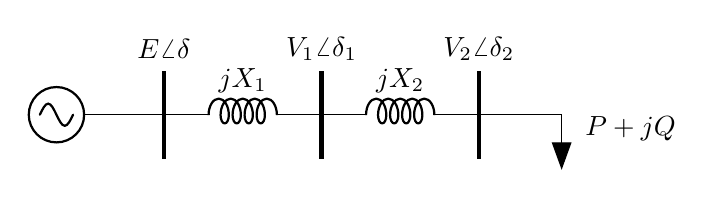
\begin{tikzpicture}[american voltages,
	scale=.7, 
	breaker/.style={rectangle,draw=black,fill=white},
	load/.style={-{Triangle[length=3.5mm,width=2.5mm,open,fill=black]}},
	node distance = 2 cm and 2 cm]
	
	% coordinate def
	\node[gen] (G1) at (0,0){};
	\coordinate[right = 1cm of G1] (B0) {};
	\coordinate[right =  of B0] (B1) {};
	\coordinate[right =  of B1] (B2) {};
	
	% bus lines
	\foreach \a in {0, 1, 2}
	\draw[ultra thick] ([yshift=-0.8cm]B\a.south) -- ([yshift=+0.8cm]B\a.north);
	
	% connecting lines
	\draw (G1) -- (B0);
	\draw (B0) to [L, l=$jX_1$] (B1);
	\draw (B1) to [L, l=$jX_2$] (B2);
	
	% Bus voltage labels
	\draw ($(B0) +(0,+1.2)$) node {$E \angle \delta$}; % ($(B0) +(0,+1.2)$) calculates location 1.2 cm above B0
	\draw ($(B1) +(0,+1.2)$) node {$V_1 \angle \delta_1$};
	\draw ($(B2) +(0,+1.2)$) node {$V_2 \angle \delta_2$};
	
	% load
	\coordinate (load1) at ($ (1.5,-1 ) + (B2)$) {}; %placement of load
	\draw[load] (B2) -| (load1) {} ; % drawing of load
	% load label Label
	\draw ($(load1)+(1.25,0.75)$) node {$P+jQ$};
	\end{tikzpicture}
	
\end{document}